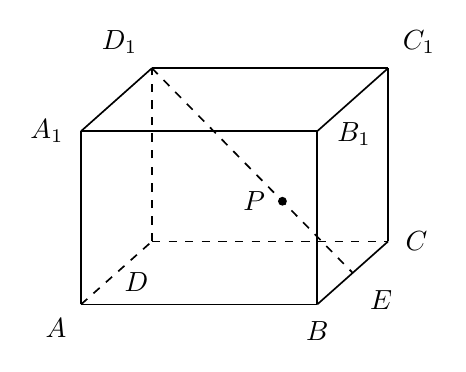
\begin{tikzpicture}[line width=0.6pt, font=\normalsize, inner sep=1pt]
\coordinate (A) at (0,0);
\coordinate (B) at (3,0);
\coordinate (B1) at (3,2.2);
\coordinate (A1) at (0,2.2);
\coordinate (D) at (0.9,0.8);
\coordinate (C) at (3.9,0.8);
\coordinate (D1) at (0.9,3);
\coordinate (C1) at (3.9,3);
\coordinate (E) at (3.45,0.4);
\coordinate (P) at (2.5575,1.31);
% solid visible edges
\draw (A) -- (B);
\draw (B) -- (B1);
\draw (B1) -- (A1);
\draw (A1) -- (A);
\draw (A1) -- (D1);
\draw (D1) -- (C1);
\draw (C1) -- (C);
\draw (C1) -- (B1);
\draw (B) -- (C);
% hidden / interior edges
\draw[dashed] (A) -- (D);
\draw[dashed] (D) -- (C);
\draw[dashed] (D) -- (D1);
\draw[dashed] (D1) -- (E);
% point P on segment D1E
\fill (P) circle (1.6pt);
% labels placed clear of strokes
\node[below left=4pt] at (A) {$A$};
\node[below=5pt] at (B) {$B$};
\node[right=5pt,xshift=1pt,yshift=-1pt] at (B1) {$B_{1}$};
\node[left=5pt] at (A1) {$A_{1}$};
\node[below left=5pt,xshift=5pt,yshift=-5pt] at (D) {$D$};
\node[right=5pt] at (C) {$C$};
\node[above left=4pt] at (D1) {$D_{1}$};
\node[above right=4pt] at (C1) {$C_{1}$};
\node[below right=5pt] at (E) {$E$};
\node[left=5pt] at (P) {$P$};
\end{tikzpicture}
